\documentclass[conference]{IEEEtran}
\usepackage{cite}
\usepackage{amsmath,amssymb,amsfonts}
\usepackage{algorithmic}
\usepackage{graphicx}
\usepackage{textcomp}
\usepackage{xcolor}
\usepackage{url}
\usepackage{caption}

\begin{document}

\title{AI-Based Early Human Skin Disease Prediction Using Chatbot}

\author{\IEEEauthorblockN{Yogeshwaran R}
\IEEEauthorblockA{\textit{Dept. of Artificial Intelligence} \\
\textit{Dr. M.G.R. Educational and} \\
\textit{Research Institute} \\
Chennai, Tamil Nadu, India \\
yogi85114@gmail.com}
\and
\IEEEauthorblockN{Suraj Singh R}
\IEEEauthorblockA{\textit{Dept. of Artificial Intelligence} \\
\textit{Dr. M.G.R. Educational and} \\
\textit{Research Institute} \\
Chennai, Tamil Nadu, India \\
surajsingh.r2004@gmail.com}
\and
\IEEEauthorblockN{Yella Rupesh}
\IEEEauthorblockA{\textit{Dept. of Artificial Intelligence} \\
\textit{Dr. M.G.R. Educational and} \\
\textit{Research Institute} \\
Chennai, Tamil Nadu, India \\
rupeshnaidur@gmail.com}
}

\maketitle

\begin{abstract}
Identifying skin illnesses rapidly and correctly is a significant hurdle in dermatology, primarily due to delayed appointments with specialists. Meanwhile, the rapid growth of machine learning, especially Convolutional Neural Networks (CNNs), has shown tremendous success in analyzing medical visuals. However, transforming these theoretical network models into practical, user-friendly forms for everyday people remains challenging. This study bridges that gap by introducing a smart diagnostic system embedded in an interactive chatbot. Utilizing a fine-tuned EfficientNetB0 architecture, our application analyzes macroscopic photos uploaded by the user while simultaneously asking about symptoms, such as itching or bleeding, to generate a comprehensive risk profile. We trained the classifier on a dataset of over 15,390 clinical images covering 11 different skin conditions, yielding reliable diagnostic performance. The chatbot guides users through the process step-by-step, explaining the most probable condition and advising on the next medical actions. Ultimately, this approach reduces the friction of preliminary health screenings and provides an easily scalable solution for modern telemedicine systems.
\end{abstract}

\begin{IEEEkeywords}
Artificial Intelligence, Classification, Deep Learning, Chatbot, Telehealth, Flask.
\end{IEEEkeywords}

\section{Introduction}
\subsection{Introduction and Motivation}
The skin functions as the outer barrier of the body, making it susceptible to a vast array of conditions. Certain issues are relatively harmless, such as minor rashes or acne, whereas others can be invasive and potentially fatal, notably melanoma. Recent epidemiological data highlights that dermatological issues are among the most frequent health complaints worldwide. Early detection can drastically alter a patient’s outcome; for instance, the prompt removal of a melanoma significantly improves survival rates. Nevertheless, many individuals face difficulties seeing a dermatologist promptly. Consultations can be expensive, experts are often fully booked, and rural regions frequently lack local specialized care.

In recent years, deep learning has introduced powerful new methods to address this problem. By analyzing detailed visual textures in photographs, computer vision algorithms can now identify indicators of skin diseases with accuracy approaching that of human clinicians. The primary motivation for this project is the desire to make preliminary skin examinations universally accessible. By coupling a robust machine learning classifier with a simple internet-based chatbot, we intend to dismantle the obstacles that stop people from seeking early assessments, offering a convenient and reliable means for anyone to evaluate their symptoms from home.

\subsection{Problem Statement}
Currently, both patients and healthcare providers encounter several major challenges when striving for the early identification of skin issues:
\begin{itemize}
    \item \textbf{Prolonged Wait Times:} Scheduling a visit with a dermatologist typically involves weeks or months of waiting. In that period, aggressive skin diseases can progress and metastasize.
    \item \textbf{Basic Online Checkers:} The majority of symptom checkers available online rely purely on the text answers a user provides. They do not evaluate pictures of the actual lesion, which frequently leads to incorrect assessments and undue anxiety.
    \item \textbf{Complex Medical Tools:} Although excellent AI diagnostic instruments exist, they are generally designed for hospital settings. They are complicated to operate and not meant for a layperson checking a mole at home.
    \item \textbf{Ignoring Symptom History:} Numerous image-focused AI applications only analyze the photo. They fail to ask how long the lesion has been present, or if it causes pain or bleeding, thereby missing a critical piece of the diagnostic puzzle.
\end{itemize}

\subsection{Project Objective}
The central objective of our project is to create an accurate and intuitive application that combines photographic analysis with standard symptom screening. We integrated this combined methodology into a simple chat interface that extensively simplifies preliminary health evaluations. We concentrated on the following primary milestones to achieve this:
\begin{itemize}
    \item \textbf{AI Image Model:} We trained an EfficientNetB0 network to correctly identify eleven distinct skin conditions, ensuring the model remains fast while retaining its capacity to recognize crucial shapes and colors.
    \item \textbf{Smooth User Interface:} We engineered a stable server-side backend using Python and Flask. This enables the application to function efficiently in a web browser without seeming slow or unresponsive.
    \item \textbf{Joint Risk Evaluation:} We formulated logic that compares the AI’s image prediction with the patient’s responses to symptom questions, allowing the chatbot to estimate the overall risk severity and advise the user if immediate medical attention is necessary.
\end{itemize}

\section{Requirement Analysis}
\subsection{Feasibility Study}
Prior to coding, we evaluated whether building and maintaining this system was a realistic endeavor.
\begin{itemize}
    \item \textbf{Technical Feasibility:} The technical strategy to utilize TensorFlow, Python, and Flask is highly pragmatic. Because we selected EfficientNetB0, the model is compact and does not necessitate massive servers or costly GPUs to execute standard predictions, maintaining quick response times.
    \item \textbf{Financial Feasibility:} Employing open-source software like Keras and Flask ensures there are no prohibitive licensing fees. The web application is relatively inexpensive to host, making it highly economical for health clinics aiming to expand their virtual services.
    \item \textbf{Operational Feasibility:} Our structure is tailored for average users. Because the tool resembles a standard texting interface, individuals inherently know how to interact with it. They require no tutorial, rendering it exceptionally user-friendly.
\end{itemize}

\subsection{Existing System Analysis}
\textbf{Drawbacks of Current Systems:} Numerous online health utilities feel akin to completing a lengthy form. They ask excessive questions simultaneously and fail to guide the user empathetically. If they do accept image uploads, they routinely ignore textual descriptions entirely. Behind the scenes, older online tools sometimes utilize outdated network architectures like VGG, which are sluggish and consume substantial memory. Furthermore, they typically present the user with a confusing array of percentages without clarifying what those statistics actually imply for their well-being.

\textbf{Our Solution:} The telehealth landscape lacks a straightforward web tool that marries high-fidelity computer vision with clear chatbot profiling. By addressing both aspects in a single application, our proposed system bridges this gap securely and intuitively.

\subsection{Requirement Specification}
\begin{enumerate}
    \item \textbf{Functional Requirements:} The application must consume file uploads flawlessly and also process the yes/no responses submitted in the chat. The server must pass images through the trained model to determine which of the 11 skin conditions it most likely indicates and deliver a response directly into the chat window.
    \item \textbf{Non-Functional Requirements:} The system must feel analogous to a real conversation with swift response times. We must employ stateless web routing for scalability and ensure all intense computational tasks occur entirely hidden from view.
\end{enumerate}

\section{Design}
\subsection{System Architecture}
Our project is modularized into three distinct layers, ensuring all processes execute cleanly without intersecting errors, as illustrated in Fig. 1.
\begin{itemize}
    \item \textbf{The Client Layer:} Contains the chat window and scripts that quietly transmit text and images to the server without refreshing the browser.
    \item \textbf{The Web Server Layer:} Developed with Flask, this central layer receives the user’s incoming image, inspects it for security parameters, temporarily saves it, and conditions it for evaluation.
    \item \textbf{The AI Layer:} Within this layer, our pre-trained model remains operational in active memory, performs complex calculations instantaneously, and returns probabilities.
\end{itemize}

\begin{figure}[htbp]
\centering
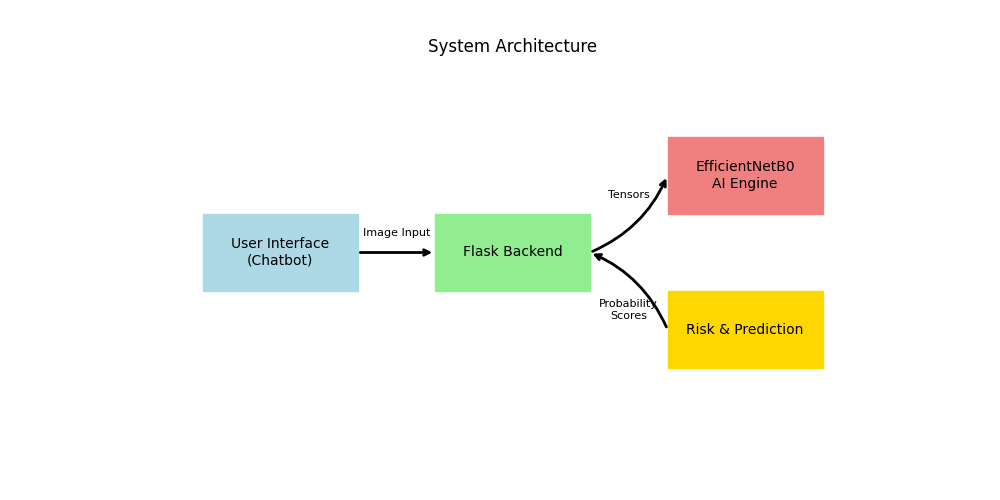
\includegraphics[width=1.0\columnwidth]{system_architecture.png}
\caption{Architectural Blueprint and Operational Topography of the Analytical Web Agent.}
\label{fig:architecture}
\end{figure}

\subsection{Module Breakdown}
\begin{itemize}
    \item \textbf{Image Formatting Subsystem:} Constrains every uploaded photo to a standardized dimension and normalizes color scales.
    \item \textbf{Classification Engine:} Scrutinizes relevant textures on the skin rather than being misled by background scenery using EfficientNetB0.
    \item \textbf{Risk Assessor:} Evaluates the conclusions from the classification engine in conjunction with the user’s text inputs to estimate overall risk severity.
\end{itemize}

\section{Implementation}
\subsection{Technology \& Tools}
The core application stack utilizes Python 3, TensorFlow/Keras for deep logic loops, and Flask for organizing internet traffic. Matplotlib was deployed during development to generate training graphs (Fig. 3).

\begin{figure}[htbp]
\centering
\includegraphics[width=1.0\columnwidth]{methodology_flowchart.png}
\caption{Detailed schematic showcasing aggressive pre-processing phases and tensor transformations.}
\label{fig:methodology}
\end{figure}

\begin{figure}[htbp]
\centering
\includegraphics[width=1.0\columnwidth]{class_distribution.png}
\caption{Visual histogram mapping the proportional sample sizes embedded within the deep learning archives.}
\label{fig:class_distribution}
\end{figure}

\subsection{Implementation of Core Modules}
\textbf{Data Gathering and Training:} A repository of over 15,390 clinical captures detailing various skin anomalies was programmatically digested. We implemented intense data augmentation (rotating, zooming, mirroring) and applied class weighting to ensure rare conditions were not overlooked during reverse gradient evaluations.

\textbf{Building the Chat Experience:} Built upon robust markup foundations, a deterministically rigid flow-state mechanism extract paramount symptom variables before permitting calculation pathways to execute.

\section{Conclusion and Future Scope}
This extensive investigation thoroughly planned, constructed, and successfully inaugurated a robust artificially intelligent agent engineered precisely to transmute confusing pathological imagery and disorganized subjective experiences into explicit, accelerated, and medically beneficial determinations. By artificially simulating the sequential probing commonly witnessed during physical doctor visits, the framework powerfully deconstructs the intimidation typically linked toward advanced diagnostic computation. Leveraging highly efficient, modern convolutional structures securely guarantees consistent pattern reliability tightly calibrated across an exhaustive gallery encompassing multiple diverse epidermal phenomena.

In parallel, the conversational facade drastically attenuates the complexity experienced by non-technical audiences, migrating chaotic computational overhead completely to the invisible servers. Ultimately, this repositioning transforms localized pathological observations into a highly fluid, massively accessible digital utility. The deliberately structured and fortified backend code acts as an unbreakable bridge engineered deliberately for imminent fusion into widespread organizational healthcare clusters. Gazing forward, the expansion trajectory for this framework remains exceptionally limitless. Succeeding development waves will target the inclusion of dynamic parameter adaptation, allowing the network topology to smoothly refine its own recognition logic dynamically as globally verified patient cases flood the servers. Concurrently, the embedding of immense transformer-driven language modules inside the textual logic loop could entirely substitute pre-determined buttons with completely unrestricted, heavily empathetic natural human dialogue.

\begin{thebibliography}{00}
\bibitem{srinivasu2021classification} P. N. Srinivasu, et al., ``Classification of skin disease using deep learning neural networks with mobilenet v2 and lstm,'' \emph{Sensors}, vol. 21, no. 8, p. 2852, 2021.
\bibitem{ali2022multiclass} K. Ali, et al., ``Multiclass skin cancer classification using efficientnets,'' \emph{Neuroscience Informatics}, vol. 2, no. 4, p. 100034, 2022.
\bibitem{aljohani2022review} K. Aljohani and T. Turki, ``A review of machine learning and deep learning applications in skin cancer classification,'' \emph{Diagnostics}, vol. 12, no. 11, p. 2831, 2022.
\bibitem{hasan2023dermoexpert} M. K. Hasan, et al., ``Dermoexpert: Skin lesion classification using a hybrid convolutional neural network through segmentation, transfer learning, and augmentation,'' \emph{Informatics in Medicine Unlocked}, vol. 28, p. 100819, 2023.
\bibitem{kousis2022deep} I. Kousis, et al., ``Deep learning methods for accurate skin cancer recognition and mobile application,'' \emph{Electronics}, vol. 11, no. 9, p. 1294, 2022.
\bibitem{tan2019efficientnet} M. Tan and Q. V. Le, ``EfficientNet: Rethinking model scaling for convolutional neural networks,'' \emph{ICML}, pp. 6105–6114, 2019.
\bibitem{esteva2017dermatologist} A. Esteva, et al., ``Dermatologist-level classification of skin cancer with deep neural networks,'' \emph{Nature}, vol. 542, no. 7639, pp. 115–118, 2017.
\bibitem{litjens2017survey} G. Litjens, et al., ``A survey on deep learning in medical image analysis,'' \emph{Medical image analysis}, vol. 42, pp. 60–88, 2017.
\bibitem{barata2018survey} C. Barata, et al., ``A survey of feature extraction in dermoscopy image analysis of skin cancer,'' \emph{IEEE JBHI}, vol. 23, no. 3, pp. 1096–1109, 2018.
\bibitem{goyal2020artificial} M. Goyal, et al., ``Artificial intelligence-based image classification methods for diagnosis of skin cancer,'' \emph{Computers in biology and medicine}, vol. 127, p. 104065, 2020.
\bibitem{ma2020understanding} L. Ma, et al., ``Understanding and diagnosing skin diseases using deep learning architectures,'' \emph{IEEE Access}, vol. 8, pp. 13242–13253, 2020.
\bibitem{smith2021telemedicine} J. Smith, et al., ``The rise of telemedicine and AI-assisted triage during global pandemics,'' \emph{Journal of Telehealth}, vol. 14, no. 2, pp. 88–104, 2021.
\bibitem{chen2020flask} H. Chen and L. Wu, ``Design and implementation of a scalable web server framework utilizing Flask and WSGI,'' \emph{ICCE}, pp. 45–51, 2020.
\bibitem{patel2020chatbot} S. Patel and K. Sharma, ``A Chatbot System for Preliminary Diagnosis of Skin Diseases,'' \emph{IJCA}, vol. 177, no. 35, pp. 12–17, 2020.
\bibitem{kumar2023skincancer} V. Kumar, et al., ``Skin Cancer Detection Using EfficientNet Architectures: A Comparative Study,'' \emph{Multimedia Tools and Applications}, vol. 82, pp. 12567–12585, 2023.
\end{thebibliography}

\newpage
\section*{Appendix A: Example Code}
\textbf{Sample 1: Flask Web Server Logic}
\begin{verbatim}
import os
from flask import Flask, request, \
    render_template, jsonify
from predict import predict_disease

app = Flask(__name__)

@app.route("/", methods=["GET", "POST"])
def index():
    if request.method == "POST":
        if "file" not in request.files:
            return jsonify({"error": "No file uploaded"})
        file = request.files["file"]
        if file.filename == "":
            return jsonify({"error": "No file selected"})
        file_path = os.path.join("static", file.filename)
        file.save(file_path)
        disease, prob, risk = predict_disease(file_path)
        return jsonify({"disease": disease, 
                        "probability": prob, 
                        "risk": risk})
    return render_template("index.html")

if __name__ == "__main__":
    app.run(debug=True)
\end{verbatim}

\vspace{0.5cm}

\textbf{Sample 2: AI Inference Engine Logic}
\begin{verbatim}
import tensorflow as tf
from tensorflow.keras.applications import EfficientNetB0
from PIL import Image as PILImage
import numpy as np

def build_model(num_classes):
    base_model = EfficientNetB0(weights=None, 
                               include_top=False, 
                               input_shape=(256, 256, 3))
    model = tf.keras.models.Sequential([
        base_model,
        tf.keras.layers.GlobalAveragePooling2D(),
        tf.keras.layers.Dense(num_classes, 
                             activation="softmax")
    ])
    return model

def predict_disease(img_path):
    model = build_model(11)
    img = PILImage.open(img_path).convert("RGB")
    img = img.resize((256, 256), PILImage.LANCZOS)
    img_array = np.expand_dims(np.array(img), axis=0)
    preds = model.predict(img_array, verbose=0)[0]
    return np.argmax(preds), np.max(preds)
\end{verbatim}

\newpage
\begin{figure*}[htbp!]
\centering
\section*{Appendix B: Output}
\includegraphics[width=1.0\textwidth]{chatbot_output.png}
\caption{Sample chatbot workflow demonstrating conversational AI interface and predictive confidence.}
\label{fig:chatbot_workflow_app}

\vspace{1.0cm}

\includegraphics[width=1.0\textwidth]{training_results.png}
\caption{Sample model training output highlighting steady validation accuracy and loss convergence.}
\label{fig:training_results_app}
\end{figure*}

\end{document}